\chapter{CONCLUSION AND FUTURE LINES}
\label{ch:Conclusion and Future Lines}

\section{Conclusion}
To conclude this work we can say that the algorithm to open the envelope works correctly. The spiral movement is a good approach to plan the trajectory of the end enfector in order to unwound the string form the circular pivots. We have demonstrated that it is possible for a robot to open a string-envelope only with a wrist force/torque sensor. Furthermore, even if the algorithm is not perfect, it succeeds more than an average human in the same conditions.

\section{Future Lines}
In order to continue developing this project, we could add corrective movements. We saw that when humans succeeded to open the envelope, it was because they were able to correct their movement. If we add corrective movements to the robot, its percentage of success could increase.

We also noticed that when humans opened the envelope correctly, they did it in less time than the robot. The speed of the robot's movement can be increased to such point that it could be much faster than a human. We could add superhuman capabilities to the robot by increasing its speed, so it would open the envelope in less than 5 seconds.

In order to enhance autonomy, other sensors such as visual sensing could be added to the robot. If we provide the robot with visual sensing, it could for example detect the end of the string at the beginning and grasp it, or measure the distance between pivots and pivots' radius. This way, we would get rid of the preconditions we have and the algorithm would become more general and work in many different situations and with different parameters of envelopes.

Finally, we created a project on GitHub (Figure~\ref{fig:github}). This is a platform for collaborative development that contains from open source projects to private team repositories. There, developers can discover, share, and build better software. The repository created for this project is called "envelope" and it can be found in the following link: https://github.com/irunegoizueta/envelope/. There, we can find all the executables needed for the algorithm to work correctly and an explanation of how to install and run them.
\begin{figure}[htbp]
	\centering
	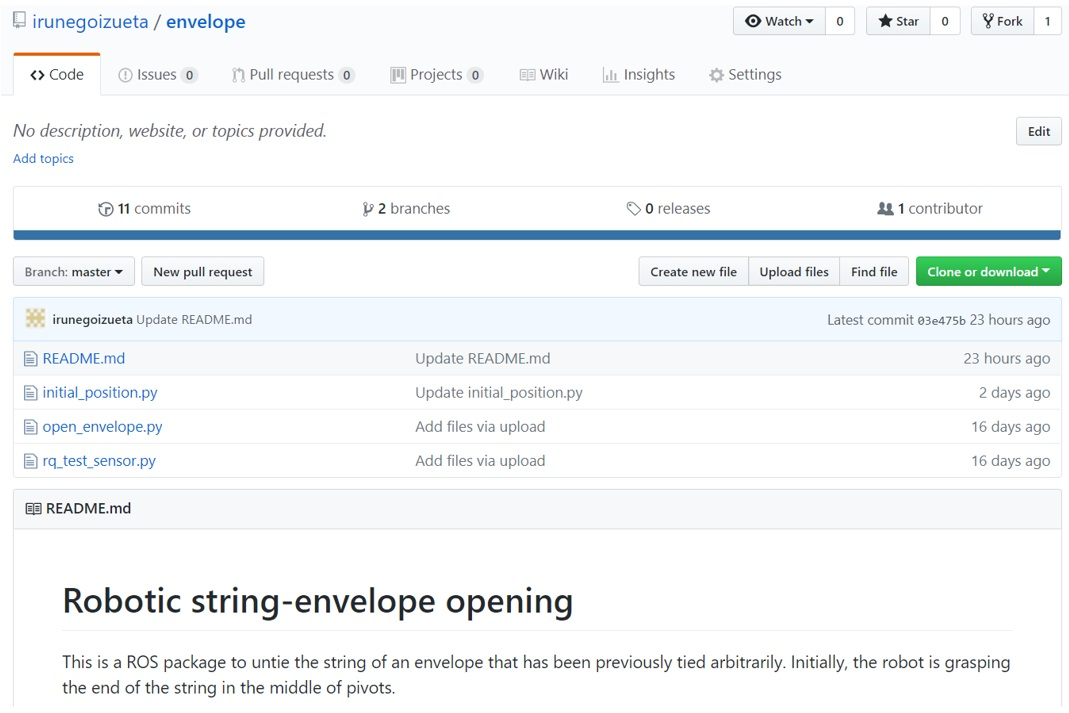
\includegraphics[height=110mm]{chapters/figures/conclusion/github.jpg}
	\caption{Repository "envelope" on GitHub.}
	\label{fig:github}
\end{figure}
